\documentclass[12pt,a4paper]{article}
\usepackage[T1]{fontenc}
\usepackage[utf8]{inputenc}
\usepackage[ngerman]{babel}
\usepackage[a4paper,margin=14mm]{geometry}
\usepackage{lmodern}
\usepackage[table]{xcolor}
\usepackage{tabularx}
\usepackage{amsmath}
\usepackage{microtype}
\usepackage{tikz}
\usepackage{graphicx}
\usetikzlibrary{arrows.meta,calc}
\newif\ifsolution
\solutiontrue
\pagestyle{empty}
\setlength{\parindent}{0pt}
\setlength{\parskip}{0pt}
\renewcommand{\familydefault}{\sfdefault}
\definecolor{Navy}{HTML}{17324D}
\definecolor{Blue}{HTML}{3B6EA5}
\definecolor{Sky}{HTML}{EAF3FA}
\definecolor{Gold}{HTML}{F3B33D}
\definecolor{Ink}{HTML}{1E2935}
\definecolor{Muted}{HTML}{617080}
\definecolor{Line}{HTML}{D8E1E8}
\color{Ink}
\newcommand{\vB}{v_{\mathrm B}}
\newcommand{\FZ}{F_{\mathrm Z}}
\newcommand{\FG}{F_{\mathrm G}}
\newcommand{\FS}{F_{\mathrm S}}
\newcommand{\kopf}[1]{%
  \colorbox{Navy}{\parbox{\dimexpr\linewidth-2\fboxsep\relax}{%
    \vspace{1.0mm}\color{white}
    \begin{tabularx}{\linewidth}{@{}Xr@{}}
      {\small\bfseries PHYSIK \textperiodcentered{} KLASSE 11} &
      \colorbox{Gold}{\color{Navy}\small\bfseries\strut\ifsolution LÖSUNGEN\else ÜBUNGSBLATT\fi}
    \end{tabularx}
    \vspace{0.7mm}
    {\fontsize{16}{19}\selectfont\bfseries Übungsblatt zur Schulaufgabe}\par
    \vspace{0.3mm}{\small #1}\vspace{0.8mm}
  }}\par\vspace{1.5mm}}
\newcommand{\frage}[2]{%
  \vspace{5mm}{\color{Blue}\bfseries\large #1 \textperiodcentered{} #2}\par
  \vspace{0.2mm}{\color{Blue}\rule{\linewidth}{0.65pt}}\par\vspace{0.8mm}}
\newcommand{\tip}[2][.86\linewidth]{%
  \par\noindent\makebox[\linewidth][c]{\rotatebox[origin=c]{180}{%
    \tikz[baseline=(b.base)]\node[draw=Blue,fill=Sky,rounded corners=2mm,line width=.7pt,
      inner sep=2mm,text width=#1,align=center,font=\normalsize,text=Ink](b){#2};}}\par\vspace{0.4mm}}
\newcommand{\rasterfeld}[2]{%
  \par\vspace{0.7mm}\noindent
  \begin{tikzpicture}[x=1mm,y=1mm]
    \pgfmathsetmacro{\rw}{\linewidth/1mm-1}
    \path[use as bounding box] (0,0) rectangle (\rw,-#1);
    \draw[step=5mm,Line!78,line width=.25pt] (0,0) grid (\rw,-#1);
    \draw[Line,line width=.55pt] (0,0) rectangle (\rw,-#1);
    \ifsolution
      \node[anchor=north west,text width=\dimexpr\linewidth-3mm\relax,inner sep=0pt,
        align=left,font=\fontsize{12}{14.4}\selectfont,text=Blue] at (1.2,-1.2) {#2};
    \fi
  \end{tikzpicture}\par}
\newcommand{\fuss}[1]{%
  \vfill{\color{Line}\rule{\linewidth}{0.5pt}}\par\vspace{1mm}
  \begin{tabularx}{\linewidth}{@{}Xr@{}}
    {\small\color{Muted}Klasse 11 \textperiodcentered{} Physik \textperiodcentered{} Kreisbewegungen} &
    {\small\color{Muted}\ifsolution Lösungen\else Übungsblatt\fi{} \textperiodcentered{} Seite #1 von 3}
  \end{tabularx}}
\newcommand{\drehscheibe}{%
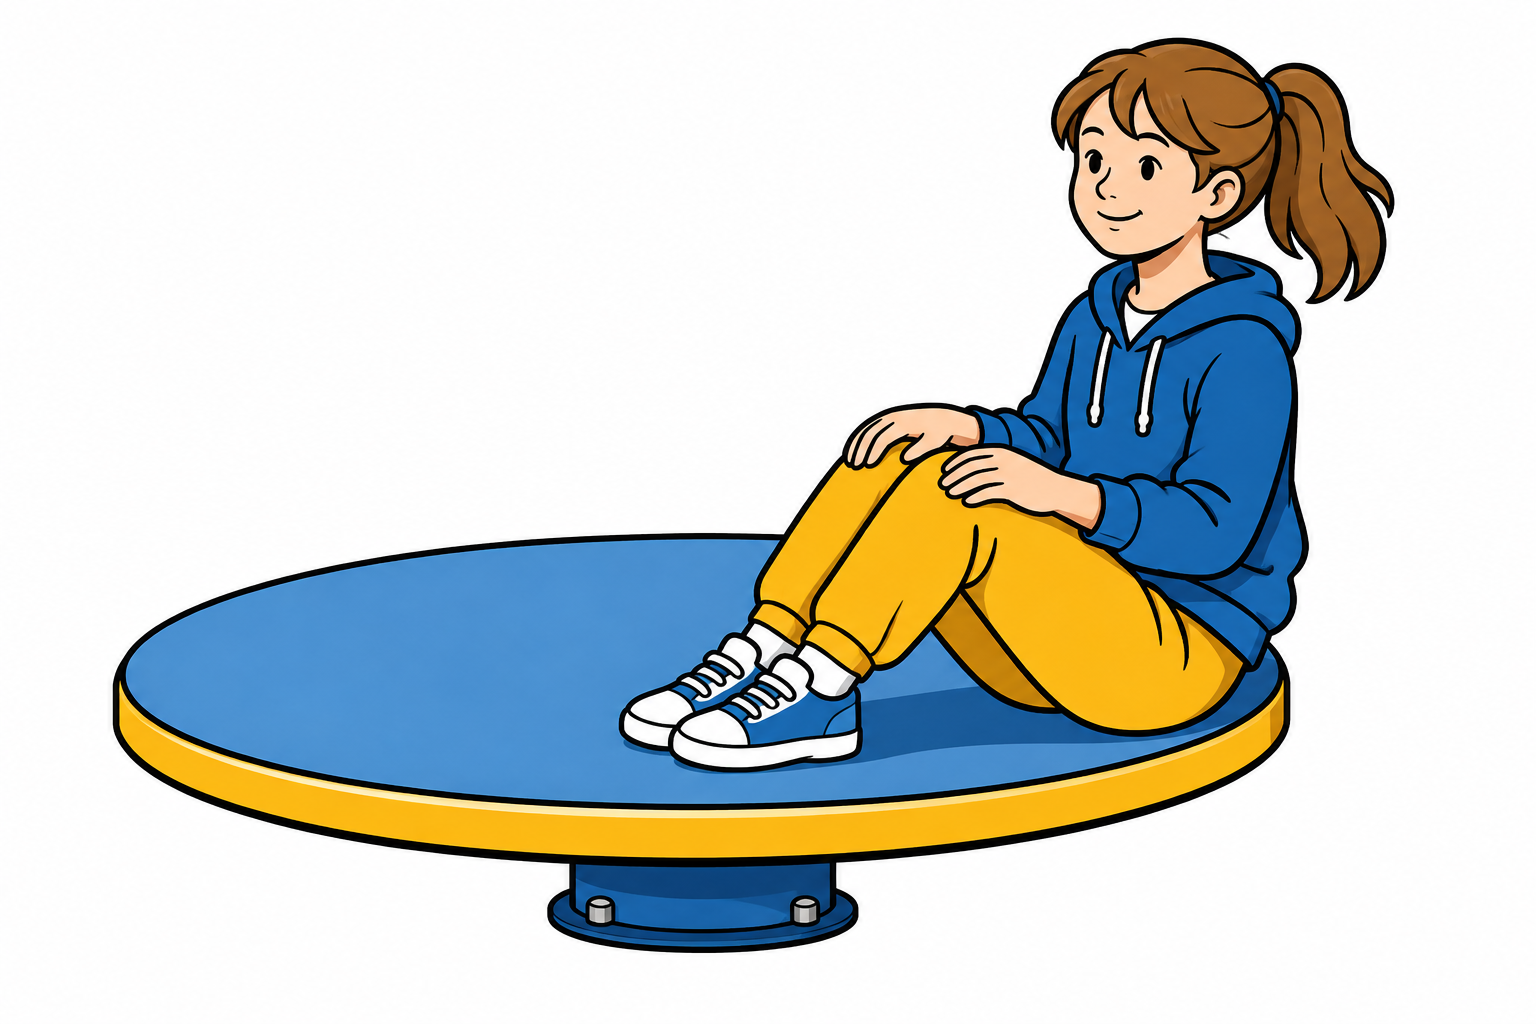
\includegraphics[width=\linewidth]{../1-Kreisbewegungen/assets/uebungsblatt-schulaufgabe/drehscheibe-kind.png}}
\newcommand{\karussell}{%
\begin{tikzpicture}[x=.70mm,y=.70mm,>=Latex,font=\small]
  \path[use as bounding box] (0,0) rectangle (135,92);
  \draw[step=7.14,Line!78,line width=.25pt] (0,0) grid (135,92);
  \draw[Line,line width=.55pt] (0,0) rectangle (135,92);
  \coordinate (A) at (27,87); \coordinate (H) at (42,81); \coordinate (P) at (87,51);
  \draw[Navy,line width=1pt] (27,5)--(27,87);
  \draw[Navy,line width=1.2pt] (19,87)--(35,87);
  \draw[Navy,line width=1.2pt] (27,81)--(42,81);
  \draw[Muted,dashed,line width=.6pt] (H)--(42,5);
  \draw[Blue,line width=1pt,fill=Sky] (79,48) rectangle (95,54);
  \draw[Ink,line width=1.4pt] (H)--(P);
  \fill[Navy] (P) circle (1.5);
  \node[font=\scriptsize,anchor=east,align=right] at (24,11) {Drehachse};
  \node[font=\scriptsize,anchor=west] at (99,52) {Kind und Sitz};
  \draw[Muted,dashed,line width=.6pt] (27,51)--(87,51);
  \node[font=\scriptsize,anchor=south] at (57,52) {$r$};
  \draw[Blue,line width=.7pt] (42,73) arc[start angle=-90,end angle=-33.7,radius=8];
  \node[Blue,font=\small] at (49,70) {$\alpha$};
  \ifsolution
    \draw[-{Latex[length=2.6mm]},Navy,line width=1.2pt] (P)--(87,21) node[right=1pt] {$\FG$};
    \draw[-{Latex[length=3.4mm,width=2.5mm]},Gold!65!Ink,line width=2.1pt] (P)--(H)
      node[midway,above=3pt,sloped,fill=white,inner sep=1pt,text=Gold!55!Ink] {$\FS$};
    \draw[-{Latex[length=2.6mm]},Navy,line width=1.3pt] (P)--(42,51) node[midway,below=1pt] {$\FZ$};
    \draw[Muted,densely dashed,line width=.8pt] (H)--(42,51) (87,21)--(42,51);
  \fi
\end{tikzpicture}}
\begin{document}
\kopf{Kreisbewegungen \textperiodcentered{} Üben und sichern}

\frage{1}{Bahngeschwindigkeit auf der Drehscheibe}
\begin{minipage}[t]{0.62\linewidth}
\vspace{0pt}
Ein Kind sitzt am Rand einer waagerechten Drehscheibe und hält sich nicht fest. Die Drehscheibe hat einen Radius von 0,80 m und dreht sich 20 Mal pro Minute.\par
\textbf{Berechne} den Betrag der Bahngeschwindigkeit, mit der das Kind auf der Drehscheibe unterwegs ist.
\par\vspace{2mm}
\tip[60mm]{Tipp: $\omega = \dfrac{2\pi}{T} = 2\pi \cdot f$}
\end{minipage}\hfill
\begin{minipage}[t]{0.34\linewidth}\vspace{0pt}\centering\drehscheibe\end{minipage}
\rasterfeld{36}{%
\(\begin{aligned}[t]
 f &= \dfrac{20}{60}\,\dfrac{1}{\mathrm s}=\dfrac13\,\dfrac{1}{\mathrm s}\\[0.5mm]
 \omega &= 2\pi\cdot f=\dfrac{2\pi}{3}\,\dfrac{1}{\mathrm s}\approx2{,}094\,\dfrac{1}{\mathrm s}\\[0.5mm]
 v_{\mathrm B} &= \omega\cdot r=\left(2\pi\cdot\dfrac{20}{60}\right)\cdot0{,}80\,\dfrac{\mathrm m}{\mathrm s}=1{,}6755\ldots\,\dfrac{\mathrm m}{\mathrm s}\approx1{,}7\,\dfrac{\mathrm m}{\mathrm s}
\end{aligned}\)\par\vspace{0.2mm}
Erst das Endergebnis wird auf zwei gültige Ziffern gerundet.}

\frage{2a}{Grenzgeschwindigkeit bestimmen}
Zwischen Kind und Drehscheibe gilt für die maximale Haftreibungskraft $F_{\mathrm{H,max}}=\mu\cdot F_{\mathrm G}$ mit $\mu=0{,}75$; $g=9{,}81\,\dfrac{\mathrm m}{\mathrm s^2}$. Die tatsächlich benötigte Haftreibungskraft muss nicht immer maximal sein.\par
\textbf{Berechne} die Grenzgeschwindigkeit, die das Kind gerade so aushalten würde, bevor es herunterfallen würde.
\tip{Tipp: Schau dir nochmal Lernmodul 5 Reiter 4 an, um den Ansatz für diese Aufgabe zu verstehen.}
\rasterfeld{80}{%
\begin{tabular}{@{}l@{\hspace{4mm}}r@{}l@{}}
Gleichsetzen für den Grenzfall: & $\displaystyle F_{\mathrm Z}$ & $\displaystyle {}=F_{\mathrm H}=\mu\cdot F_{\mathrm G}$\\[3mm]
Einsetzen: & $\displaystyle \dfrac{m\cdot v_{\mathrm B}^2}{r}$ & $\displaystyle {}=\mu\cdot m\cdot g$\\[3mm]
Kürzen: & $\displaystyle \dfrac{v_{\mathrm B}^2}{r}$ & $\displaystyle {}=\mu\cdot g$\\[3mm]
Umstellen und einsetzen: & $\displaystyle v_{\mathrm B}$ & $\displaystyle {}=\sqrt{\mu\cdot g\cdot r}$\\[3mm]
 & & $\displaystyle {}=\sqrt{0{,}75\cdot9{,}81\,\dfrac{\mathrm m}{\mathrm s^2}\cdot0{,}80\,\mathrm m}$\\[3mm]
 & & $\displaystyle {}=2{,}426107994\ldots\,\dfrac{\mathrm m}{\mathrm s}\approx2{,}4\,\dfrac{\mathrm m}{\mathrm s}$
\end{tabular}}
\fuss{1}
\newpage

\kopf{Kreisbewegungen \textperiodcentered{} Grenzfall und Beurteilung}
\frage{2b}{Grenzfrequenz beurteilen}
\textbf{Entscheide}, ob man aus den bekannten Angaben auch eine Grenzfrequenz der Drehscheibe berechnen kann. \textbf{Begründe} deine Entscheidung.
\rasterfeld{90}{%
\begin{tabular}{@{}r@{}l@{}}
\multicolumn{2}{@{}p{\dimexpr\linewidth-3mm\relax}@{}}{\textbf{Ja.} Die Grenzfrequenz lässt sich auch ohne Massenangabe bestimmen, denn die Masse kürzt sich bei}\\[1mm]
$\displaystyle \dfrac{m\cdot v_{\mathrm B}^2}{r}$ & $\displaystyle {}=\mu\cdot m\cdot g$\\[1mm]
\multicolumn{2}{@{}p{\dimexpr\linewidth-3mm\relax}@{}}{heraus. Statt wie bei 2a nach der Bahngeschwindigkeit umzustellen, kann}\\[1mm]
$\displaystyle v_{\mathrm B}$ & $\displaystyle {}=\omega\cdot r$\\[1mm]
\multicolumn{2}{@{}p{\dimexpr\linewidth-3mm\relax}@{}}{eingesetzt werden. Damit lässt sich die Winkelgeschwindigkeit berechnen. Aus}\\[1mm]
$\displaystyle \omega$ & $\displaystyle {}=\dfrac{2\pi}{T}$\\[1mm]
\multicolumn{2}{@{}p{\dimexpr\linewidth-3mm\relax}@{}}{mit Umlaufdauer $T$ und}\\[1mm]
$\displaystyle T$ & $\displaystyle {}=\dfrac{1}{f}$\\[1mm]
\multicolumn{2}{@{}p{\dimexpr\linewidth-3mm\relax}@{}}{lässt sich die Grenzfrequenz bestimmen.}
\end{tabular}}

\frage{2c}{Wetterbedingung beurteilen}
Heute ist der erste Tag unter 0 Grad Celsius. \textbf{Beurteile}, ob die Wetterbedingung einen Einfluss auf die Unfallgefahr der Situation hat.
\rasterfeld{85}{Frost kann die Unfallgefahr erhöhen, wenn sich Eis oder Reif auf der Drehscheibe bildet: Dann kann die Haftreibungszahl sinken, sodass $F_{\mathrm{H,max}}=\mu mg$ und damit die Grenzgeschwindigkeit kleiner werden. Wenn das Kind allerdings durch Frost vereist festkleben sollte, dann erhöht sich die Haftreibungskraft deutlich.}
\fuss{2}
\newpage

\kopf{Kreisbewegungen \textperiodcentered{} Kräfte am Kettenkarussell}
\noindent Nun geht es um ein Kettenkarussell. Kind und Sitz werden gemeinsam als ein Körper betrachtet; seine Masse, die Kettenlänge und die Aufhängung bleiben beim Vergleich gleich.\par
\frage{3a}{Kräfteparallelogramm ergänzen}
\textbf{Ergänze} die untere Skizze, indem du alle wirkenden Kräfte einzeichnest. Achte auf passende Pfeillängen.\par
\noindent Hinweis: Es soll ein Kräfteparallelogramm entstehen. Zeichne zuerst die Zentripetalkraft. Die Länge dieses Pfeils ist frei wählbar.\par
\noindent\begin{minipage}[t]{0.56\linewidth}\vspace{0pt}\centering\karussell\end{minipage}\hfill
\begin{minipage}[t]{0.41\linewidth}\vspace{0pt}
\begin{tikzpicture}[x=1mm,y=1mm]
  \path[use as bounding box] (0,0) rectangle (74,-74);
  \draw[step=5mm,Line!78,line width=.25pt] (0,0) grid (74,-74);
  \draw[Line,line width=.55pt] (0,0) rectangle (74,-74);
  \ifsolution
    \node[anchor=north west,text width=71mm,inner sep=0pt,align=left,
      font=\fontsize{12}{14.4}\selectfont,text=Blue] at (1,-1)
      {Am gemeinsamen Schwerpunkt wirken $F_{\mathrm G}$ senkrecht nach unten und $F_{\mathrm S}$ entlang der Kette zur Aufhängung. $F_{\mathrm S}$ ist länger als $F_{\mathrm G}$; ihre vertikale Komponente gleicht $F_{\mathrm G}$ aus. Das Parallelogramm ergibt $F_{\mathrm Z}$ waagerecht zur Drehachse. $F_{\mathrm Z}$ ist die Resultierende, keine zusätzliche Wechselwirkung.};
  \fi
\end{tikzpicture}\end{minipage}\par
\tip{Tipp: Schaue dir Lernmodul 6 Reiter 2 sowie Lernmodul 7 Reiter 3 an.}

\frage{3b}{Veränderung geometrisch erklären}
Die Drehzahl desselben Kettenkarussells wird erhöht; verglichen werden gleichförmige Kreisbewegungen nach dem Einschwingen. $r_0$ bezeichnet den konstanten Abstand zwischen Aufhängung und Drehachse; die Kettenlänge $l$ bleibt gleich.\par
\textbf{Erkläre} mit Hilfe einer geeigneten geometrischen Formel, wie sich Auslenkwinkel $\alpha$, $r$ und $g$ verändern, wenn die Zentripetalkraft steigt.
\tip{Tipp: Schaue dir Lernmodul 6 Reiter 2.}
\rasterfeld{40}{Es gilt $\tan\alpha=\dfrac{F_{\mathrm Z}}{F_{\mathrm G}}$. Bei gleicher Masse bleiben $F_{\mathrm G}=mg$ und $g=9{,}81\,\dfrac{\mathrm m}{\mathrm s^2}$ konstant. Größeres $F_{\mathrm Z}$ führt damit zu größerem $\tan\alpha$ und $\alpha$. Geometrisch gilt $r=r_0+l\cdot\sin\alpha$. Weil $r_0$ und $l$ gleich bleiben, wächst $r$ mit $\alpha$. $g$ bleibt unverändert.}
\fuss{3}
\end{document}
